\section{Can Zooming into Smaller Time Scale Improve Diversity?}

\subsection{Per-Component SPMD at Micro-Scale}
\label{sec:modelling_micro}

%% 1. Introduction: Zooming into 16.7 ms to extract variation
%%    1a. Explain the variation in 16.7 ms: Busy and idle period
%% 2. Explain how the equations are generated
%% 3. Explain the results
%%    3a. Explain why the solution are not correct
%% 4. Provide the reason for the bad solutions: explain underdetermined equations
%%    4a. Explain 2 variable in GPU
%%    4b. Explain 2 variable in CPU
%%    4c. Explain 4 variable 2 equations
%% 5. Conclusion: Due to underdetermined equations, the solution is infeasible

The repeating app usage across rendering intervals suggests that
we need to look inside each rendering interval in order to create multiple equations those
are diverse in phone component usage. 
Figure~\ref{fig:power_trace_candycrushturorial} shows the power draw during 
two 16.7 ms intervals for the Candy Crush Saga Menu scenario.
We can observe that there are two distinctive plateaus in each single 16.7 ms interval.
The higher one is when the GPU is in the Busy state and
the lower plateau is when the GPU is in Idle state. 
These two plateaus provide us with two sub intervals for generating two diverse equations.
We denote this as {\it SPMD at micro-scale}.
% When we are generating the equations over any interval longer than 16.7ms, we inadvertently average the power and loose state change information as shown in figure~\ref{fig:coarse_grained}.

\begin{figure*}[tp]
    \centering
     \begin{subfigure}[b]{0.32\textwidth}
         \centering
         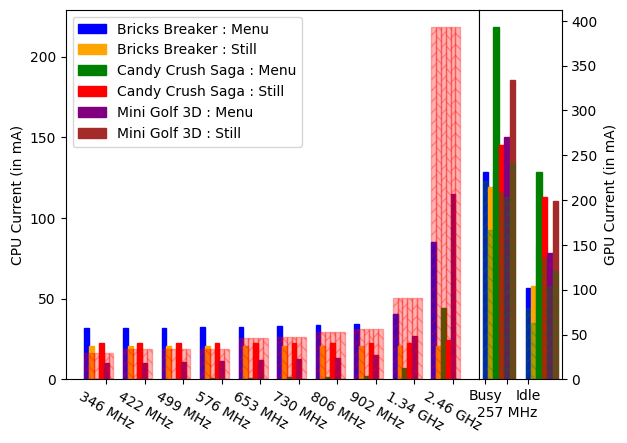
\includegraphics[width=\textwidth]{figures/002_Pixel2_16_micro_equations.png}
         \label{fig:number_parameters_vs_duration_100s_0}
     \end{subfigure}
    \begin{subfigure}[b]{0.32\textwidth}
         \centering
         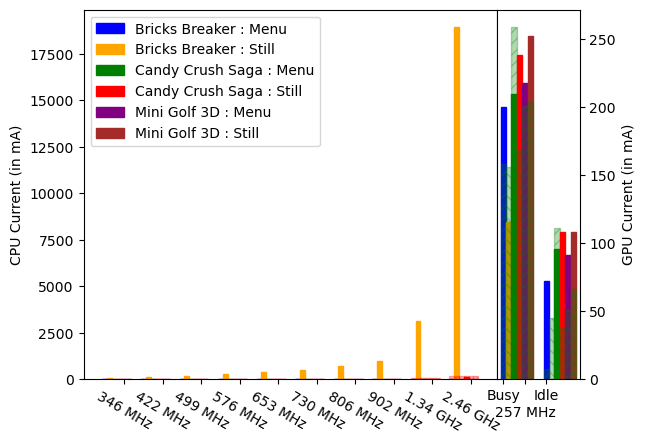
\includegraphics[width=\textwidth]{figures/003_MotoZ3_16_micro_equations.png}
         \label{fig:number_parameters_vs_duration_100s_100}
     \end{subfigure}
    \begin{subfigure}[b]{0.32\textwidth}
         \centering
         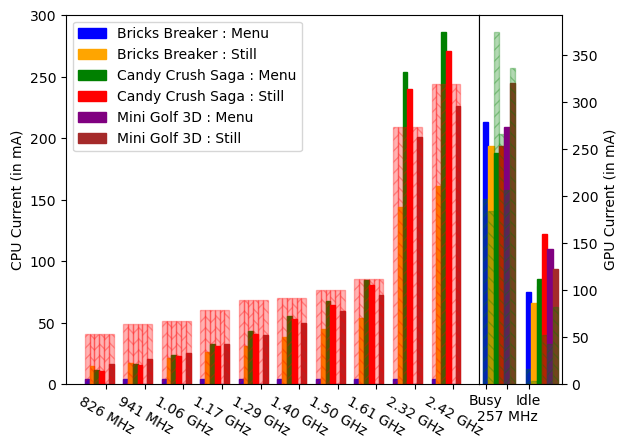
\includegraphics[width=\textwidth]{figures/004_Pixel4_16_micro_equations.png}
         \label{fig:number_parameters_vs_duration_100s_200}
     \end{subfigure}
     \hfill
     \centering
     \begin{subfigure}[b]{0.32\textwidth}
        \centering
    	{ \scriptsize
    	\begin{tabular}{ | l | c | c | c | c | c | c | }
    		\hline
    		     & \multicolumn{6}{ c|}{Error for each App Scenarios (in \%)}\\
    		\cline{2-7}
                    Model & \rot{B. Menu} & \rot{B. Still} & \rot{C. Menu} & \rot{C. Still} & \rot{M. Menu} & \rot{M. Still}  \\
    		\hline
                Fix. F. Const.       & 2.0 & 2.5 & 5.5 & 16 & 3.9 & 13 \\
                Classical            & 14 & 24 & 25 & 16 & 49 & 28 \\
    		\hline
    	\end{tabular}
    	}
	\caption{Pixel 2}
    \end{subfigure}
         \begin{subfigure}[b]{0.32\textwidth}
        \centering
    	{ \scriptsize
    	\begin{tabular}{ | l | c | c | c | c | c | c | }
    		\hline
    		     & \multicolumn{6}{ c|}{Error for each App Scenarios (in \%)}\\
    		\cline{2-7}
                    Model & \rot{B. Menu} & \rot{B. Still} & \rot{C. Menu} & \rot{C. Still} & \rot{M. Menu} & \rot{M. Still}  \\
    		\hline
                Fix. F. Const.       & 7.5 & 18 & 7.5 & 5.9 & 6.4 & 4.2 \\
                Classical            & 32 & 21 & 37 & 16 & 12 & 8.5 \\

    		\hline
    	\end{tabular}
    	}
	\caption{Moto Z3}
    \end{subfigure}
         \begin{subfigure}[b]{0.32\textwidth}
        \centering
    	{ \scriptsize
    	\begin{tabular}{ | l | c | c | c | c | c | c | }
    		\hline
    		     & \multicolumn{6}{ c|}{Error for each App Scenarios (in \%)}\\
    		\cline{2-7}
                    Model & \rot{B. Menu} & \rot{B. Still} & \rot{C. Menu} & \rot{C. Still} & \rot{M. Menu} & \rot{M. Still}  \\
    		\hline
                Fix. F. Const.       & 7.5 & 18 & 7.5 & 5.9 & 6.4 & 4.2 \\
                Classical            & 32 & 21 & 37 & 16 & 12 & 8.5 \\

    		\hline
    	\end{tabular}
    	}
	\caption{Pixel 4}
    \end{subfigure}
     \hfill
    \caption{Model parameters derived by micro-scale SPMD}
    \label{fig:micro}
    \vspace{-0.1in}
\end{figure*}

\paragraph{Methodology}
We follow the same methodology as described in \S\ref{sec:modelling_macro}
except that we generated two equations per 16.7 ms interval, one for GPU in Busy state
and the other for GPU Idle state and these correspond to the two plateaus.
As before, we fixed the base power as a constant to avoid the under-rank problem caused due to it
and use the Fix-Freq-Constrained version of the solver.


\paragraph{Findings}
In creating the two equations, we observed that there are more than two unknowns as elaborated below.
First, we observe that GPU almost never changes frequency within each 16.7ms interval,
and hence it contributes two unknowns,i.e for the GPU Busy state and Idle state power.
Second, the CPU may change frequency, potentially contributing multiple CPU power parameters.
% the active power at that multiple frequencies.
This makes the system of two equations under-determined.
%
To solve this problem, we tried to set up 2 equations 
each per interval for 2, 4, 8, 16 intervals,
% we created 8 and 32 equations for four and sixteen consecutive 16.7 ms intervals respectively.
% which typically have the same 3 unknowns as 
% the CPU ad GPU tend to stay in the same power states in generating two very similar frames.
%
% Although, we feed 4 equations into curve\_fit() to generate the solution, but they mainly
% represent only a set of 2 equations, one for GPU Active-busy and other as GPU Active-idle.
% 
Figure~\ref{fig:micro} shows the model parameters output by the regression solver for the six app scenarios on the three phones for 16 equations. The results for other 
intervals are similar and omitted due to page limit. 

We make the following observations.
(1)The power models output by the solver have LSF error
between 2.4\% to 12.8\% for Pixel 2, between 6.2\% to 15.6\% for Moto Z3 and between 2.6\% to 15.6\% for Pixel 4
(2) The individual power parameters are 1.05$\times$-1.67$\times$, 1.02$\times$-1.52$\times$, 0.94$\times$-1.44$\times$ of their counterparts  for GPU Frequency-Busy and  1.26$\times$-1.65$\times$, 0.64$\times$-4.5$\times$, 1.78$\times$-29.35$\times$ of their counterparts for GPU Frequency-Idle in the classic model for Pixel 2,Moto Z3,Pixel 4 respectively . 

% These power models are considered meaningful for use, for example, in energy accounting. 
The models are not considered acceptable as the high error suggests the models cannot capture the power state variation well. 

\paragraph{Validation}
\comment{ 
How often can we get acceptable solutions for systems of 8 equations? 
Validation of Micro SPMD using interleaved "training" and "testing" data. 
Pick 16 equations, form training data using odd equations, and testing data using even equations.
}

\if 0
(1) For most of the cases, the CPU power parameters generated are overwhelming below their
counter part in the classical model, \eg 0 mA for Boat Racing Intro with 32 equations
and close to 0 mA, \eg for Boat racing Still with 32 equations
(2) For Boat Racing Intro with 8equations, the CPU power paramaters are similar to their counterparts in the classic model, but the GPU Idle power of 161.1 mA is over 2 times higher than the corresponding 67.25 mA in the classic model. 
(3) Finally, only for two of the 12 scenarios, Bricks Breaker Intro with 8 and 32 equations, shown in bold, the power parameter seems reasonable, \ie within 50\% of their counterparts in the classic model.
\fi

\if 0
%% For Nexus 6
(3) similarly, for Nexus 6 the base power by SPMD is overestimated, 
145.2 mA and 300.7 mA for the Brick Breakers scenarios and 
419.2 mA and 413.3 mA for the Candy Crush Saga scenarios which are 7 to 21 times higher than
the 20.16 mA value in the classical model; and
(4) At 422 MHz in Bricks Breaker, 
the CPU powers are overestimated for the Intro scenario as 56.86 mA
but underestimated for the Still scenario as 8.21 mA, compare to 32.17 mA 
in the classical model.
%% 4. Provide the reason for the bad solutions: explain underdetermined equations
% Due to space constraints the detailed results are in the appendix.
\fi

\paragraph{Analysis}
To understand why some systems can generate reasonable models while other
cannot, we first plot in Table~\ref{tab:micro-rank_motoz3} the rank and top singular values for the 12 equation systems. We see that all the systems are full rank, and have sufficient number of
high singular values.  

\if 0
\begin{figure}[tp]
    \centering
    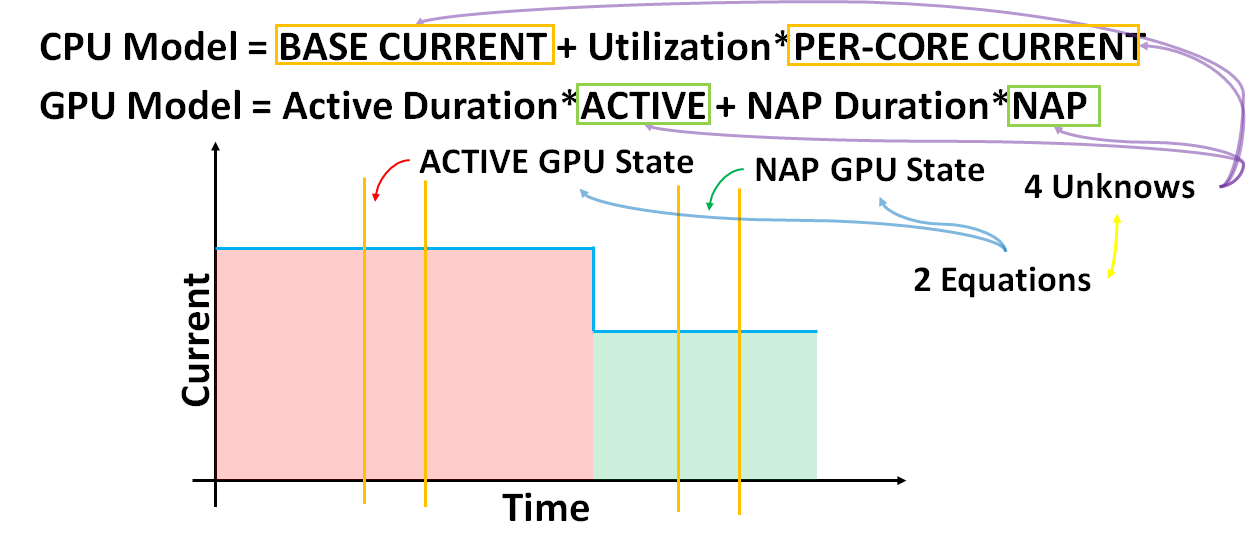
\includegraphics[width=0.95\columnwidth]{figures/underdetermined_2.png}
    \vspace{-0.1in}
    \caption{The equation are underdetermined even in 16.7 ms Micro-Scale}
    \label{fig:micro_underdetermied}
    \vspace{-0.1in}
\end{figure}
\fi

\begin{table}[tp]
{\footnotesize
    \centering
    \caption{The rank and singular values for the set of equations for micro-scale "Fix-Freq.-Constr. SPMD" for Pixel 4 for 16 equation system of equation.
    (Top 4 singular values are shown.)
    }
    \vspace{-0.1in}
    \begin{tabular}{|c|p{9mm}|p{4.5mm}|p{4.5mm}|p{4.5mm}|p{4mm}|p{4mm}|p{4mm}|p{4mm}|}
    \hline
        App & Scenario & Num. of Eqns. & Num. of Vars. & Rank &  \multicolumn{4}{c|}{Singular Values} \\
        \hline
         \multirow{2}{13mm}{Bricks Breaker} & Menu & 32 & 6 & 6 & 4.46  & 4.01  & 1.66  & 0.97 \\
         \cline{2-9}
         & Still &  32 & 6 & 6 & 4.52  & 4.02  & 1.80  & 1.01 \\
         \hline
         \multirow{2}{13mm}{Candy Crush Saga} & Menu & 32 & 7 & 7 & 5.88  & 4.02  & 3.52  & 0.56 \\
         \cline{2-9}
         & Still & 32 & 7 & 7 & 6.70  & 4.00  & 3.30  & 2.64 \\
         \hline
        \multirow{2}{13mm}{Mini Golf 3D} & Menu & 32 & 12 & 11 & 5.33  & 3.99  & 2.90  & 1.88 \\
        \cline{2-9}
	     & Still & 32 & 6 & 6 & 5.63  & 4.03  & 3.11  & 1.00 \\
	     \hline
    \end{tabular}
    \label{tab:micro-rank_motoz3}
    \vspace{-0.1in}
}
\end{table}



\begin{table}[tp]
    \centering
    \caption{Equations for the 4 consecutive 16.7 ms intervals for Bricks Breaker Menu scenario on Moto Z3.}
    {\small
    \begin{tabular}{|c|c|c|c|c|}
        \hline
             Eqn &    y(n) & \multicolumn{1}{c|}{CPU Utilization} & \multicolumn{2}{c|}{GPU Utilization} \\
        \cline{4-5}
             & (mA) & \multicolumn{1}{c|}{} & Busy & Idle \\
        \hline
                1 & 319.9 &  44\% & 100\% &   0\% \\  
                2 & 168.5 & 133\% &   0\% &  99\% \\
                \hline
                3 & 335.2 &  35\% & 100\% &   0\% \\ 
                4 & 159.8 & 131\% &   0\% &  99\% \\
                \hline
                5 & 321.4 &  86\% & 100\% &   0\% \\ 
                6 & 166.2 & 134\% &   2\% &  97\% \\
                \hline
                7 & 292.9 &  40\% & 100\% &   0\% \\ 
                8 & 162.3 & 136\% &   0\% &  99\% \\   
        \hline
    \end{tabular}
    }
    \label{tab:equations_micro}
\end{table}

Next, we take a close look at two systems, one with acceptable and one with unacceptable power parameters generated.
Table~\ref{tab:equations_micro} shows the 8 equations for 
Bricks Breaker Menu for Moto Z3 
%with 8 equations,
where equations 1, 3, 5 and 7 correspond to the GPU Busy subintervals and 
equations 2, 4, 6 and 8 correspond to the GPU Idle subintervals within the rendering intervals. 

We make two  observations:
(1) the four equations for GPU Idle subintervals, 2, 4, 6, and 8 are very similar in GPU usage
and the four equations for GPU Busy subintervals, 1, 3, 5, and 7 are very similar in GPU usage. 
(2) These two groups differ in CPU utilization which are consistent with their
the energy values on the LHS.
We see that the noise in energy values appear to dominate the diversity in CPU usage. 
For example, the CPU utilization of Eq.~.1 and Eq.~3 are 44\% and 35\%,
but their normalized energy value are 319.9 mA and 335.2 mA, respectively. 
As a result, the solver is not able to generate meaningful CPU power parameters.
\comment{
how do we explain the energy value variation
between Eq.~2 and Eq.~4  does not affect the solutions here?
}

\if 0
\comment{
Table~\ref{tab:equations_micro_bricksbreaker_still} shows the 8 equations for 
Bricks Breaker Still scenario on Moto Z3 which results in incorrect solutions, \eg CPU power of 0 mA.
We see that the noise in energy values appear to dominate the
diversity in CPU usage. 
For example, 
the CPU utilization of Eq.~.2 and Eq.~4 are 124\% and 124\%,
but their normalized energy value are 171.9 mA and 162.7 mA, respectively. 
As a result, the solver is not able to generate meaningful CPU power parameters.
}
\fi


\comment{
These results suggest while zooming into rendering intervals increased the diversity of the systems of equations - they are full rank and have good singular values, but the most of the times the solver cannot output reasonable model parameters due to energy value measurement noise. 
} \comment{not sure what to conclude here???}